\documentclass[11pt,a4paper]{article}
\usepackage[margin=2.5cm]{geometry}
\usepackage{amsmath,amssymb,amsthm}
\usepackage{xcolor}
\usepackage{tikz}
\usetikzlibrary{arrows.meta,positioning}
\usepackage{tcolorbox}
\usepackage{booktabs}
\usepackage{enumitem}

\definecolor{convblue}{RGB}{31,119,180}
\definecolor{prodgreen}{RGB}{44,160,44}
\definecolor{decred}{RGB}{214,39,40}

\newcommand{\conv}{\circledast}
\newcommand{\nprod}{\odot}
\newcommand{\xmark}{\oplus}

\title{\textbf{MAC SC Decoding from First Principles}\\[5pt]
\large How Circular Convolution and Normalized Product\\Decode Two-User Polar Codes}
\author{Tutorial Notes}
\date{}

\begin{document}
\maketitle
\thispagestyle{empty}

%==============================================================
\section{Setup}
%==============================================================

Two users $U$ and $V$ send binary messages through a shared channel.

\subsection{Polar Encoding (N=2)}
Each user encodes independently using the polar transform:
\begin{align}
x_1 &= u_1 \oplus u_2, \quad x_2 = u_2 \quad \text{(User U)} \\
y_1 &= v_1 \oplus v_2, \quad y_2 = v_2 \quad \text{(User V)}
\end{align}
where $\oplus$ is XOR (addition mod 2).

\subsection{Channel}
The channel is \textbf{memoryless across positions}: the output $z_i$ depends only on the inputs $(x_i, y_i)$ at position $i$:
\[
P(z_1, z_2 \,|\, x_1, y_1, x_2, y_2) = P(z_1 \,|\, x_1, y_1) \cdot P(z_2 \,|\, x_2, y_2)
\]

\subsection{Transition Tensors}
For each observation $z_i$, define a $2\times 2$ tensor:
\[
T_{z_i}[x, y] = P(z_i \,|\, x_i = x,\, y_i = y), \quad x,y \in \{0,1\}
\]

\begin{tcolorbox}[colback=blue!5,colframe=convblue,title=Example: GMAC at SNR = 6\,dB]
Channel: $Z_i = (1-2X_i) + (1-2Y_i) + W_i$, \; $W_i \sim \mathcal{N}(0, \sigma^2)$, \; $\sigma^2 = 0.251$.

Suppose $z_1 = 1.3$, $z_2 = -0.8$. Then:
\[
T_{z_1} = \begin{pmatrix} 0.655 & 0.107 \\ 0.107 & 0.005 \end{pmatrix}, \quad
T_{z_2} = \begin{pmatrix} 0.005 & 0.107 \\ 0.107 & 0.655 \end{pmatrix}
\]
where entry $[x,y]$ corresponds to $\mathcal{N}(z_i;\, (1\!-\!2x)+(1\!-\!2y),\, \sigma^2)$.
\end{tcolorbox}

\subsection{Goal}
From $(z_1, z_2)$, recover the message bits $(u_1, u_2, v_1, v_2)$.

%==============================================================
\section{The Two Fundamental Operations}
%==============================================================

All of MAC SC decoding is built from two operations on $2\times 2$ tensors.

\begin{tcolorbox}[colback=blue!5,colframe=convblue,title=Operation 1: Circular Convolution $(\conv)$]
Given tensors $A$ and $B$:
\[
\boxed{(A \conv B)[u,v] = \sum_{i \in \{0,1\}} \sum_{j \in \{0,1\}} A[u \oplus i,\, v \oplus j] \cdot B[i,j]}
\]
\textbf{Meaning:} ``Marginalize over unknown bits linked through XOR encoding.''

The XOR in the polar encoding creates the XOR in the indices.
\end{tcolorbox}

\begin{tcolorbox}[colback=green!5,colframe=prodgreen,title=Operation 2: Normalized Product $(\nprod)$]
Given tensors $A$ and $B$:
\[
\boxed{(A \nprod B)[u,v] = \frac{A[u,v] \cdot B[u,v]}{\displaystyle\sum_{i,j} A[i,j] \cdot B[i,j]}}
\]
\textbf{Meaning:} ``Combine two independent observations about the same variable.''

This is Bayes' rule: multiply likelihoods, normalize.
\end{tcolorbox}

%==============================================================
\section{Step 1: Decode $u_1, v_1$ (CalcLeft)}
%==============================================================

\textbf{Question:} What is $P(z_1, z_2 \,|\, u_1, v_1)$?

\textbf{Derivation:}

Start by marginalizing over the unknown $(u_2, v_2)$:
\begin{align}
P(z_1, z_2 \,|\, u_1, v_1)
&= \sum_{u_2, v_2} P(u_2, v_2) \cdot P(z_1, z_2 \,|\, u_1, v_1, u_2, v_2) \label{eq:marg}
\end{align}

Since $(u_2, v_2)$ are uniform: $P(u_2, v_2) = \tfrac{1}{4}$. Since the channel is memoryless:
\begin{align}
&= \frac{1}{4} \sum_{u_2, v_2} P(z_1 \,|\, x_1, y_1) \cdot P(z_2 \,|\, x_2, y_2) \label{eq:factor}
\end{align}

Substitute the polar encoding ($x_1 = u_1 \oplus u_2$, $y_1 = v_1 \oplus v_2$, $x_2 = u_2$, $y_2 = v_2$):
\begin{align}
&= \frac{1}{4} \sum_{u_2, v_2} T_{z_1}[u_1 \oplus u_2,\, v_1 \oplus v_2] \cdot T_{z_2}[u_2, v_2] \label{eq:conv}
\end{align}

\begin{tcolorbox}[colback=blue!5,colframe=convblue]
\textbf{Recognize:} This is exactly the circular convolution!
\[
P(z_1, z_2 \,|\, u_1, v_1) = \frac{1}{4} \cdot \big(T_{z_1} \conv T_{z_2}\big)[u_1, v_1]
\]
\end{tcolorbox}

\textbf{Numerical example:} Expanding for $[u_1=0, v_1=0]$:
\begin{align*}
(T_{z_1} \conv T_{z_2})[0,0] &= T_{z_1}[0,0] \cdot T_{z_2}[0,0] + T_{z_1}[0,1] \cdot T_{z_2}[0,1] \\
&\quad + T_{z_1}[1,0] \cdot T_{z_2}[1,0] + T_{z_1}[1,1] \cdot T_{z_2}[1,1] \\
&= 0.655 \times 0.005 + 0.107 \times 0.107 + 0.107 \times 0.107 + 0.005 \times 0.655 \\
&= 0.003 + 0.011 + 0.011 + 0.003 = 0.029
\end{align*}

Computing all four entries and picking the largest gives us $\hat{u}_1, \hat{v}_1$.

%==============================================================
\section{Step 2: Decode $u_2, v_2$ (CalcRight)}
%==============================================================

After deciding $(\hat{u}_1, \hat{v}_1)$, we want:

\textbf{Question:} What is $P(z_1, z_2 \,|\, u_2, v_2, \hat{u}_1, \hat{v}_1)$?

Since $(u_1, v_1)$ are now fixed (decided), no marginalization needed:
\begin{align}
P(z_1, z_2 \,|\, u_2, v_2, \hat{u}_1, \hat{v}_1)
&= P(z_1 \,|\, \hat{u}_1 \oplus u_2,\, \hat{v}_1 \oplus v_2) \cdot P(z_2 \,|\, u_2, v_2) \label{eq:right1}
\end{align}

This is a product of two terms, each providing independent evidence about $(u_2, v_2)$.

\subsection{Sub-step A: Extract $z_1$'s evidence via $\conv$}

Define the decision tensor: $\delta[u,v] = \begin{cases} 1 & \text{if } (u,v) = (\hat{u}_1, \hat{v}_1) \\ 0 & \text{otherwise}\end{cases}$

Then:
\begin{align}
(\delta \conv T_{z_1})[u_2, v_2] &= \sum_{i,j} \delta[i,j] \cdot T_{z_1}[i \oplus u_2,\, j \oplus v_2] \nonumber \\
&= T_{z_1}[\hat{u}_1 \oplus u_2,\, \hat{v}_1 \oplus v_2] \label{eq:shift}
\end{align}

\begin{tcolorbox}[colback=blue!5,colframe=convblue]
The circular convolution with $\delta$ \textbf{shifts the indices} of $T_{z_1}$ by the decision $(\hat{u}_1, \hat{v}_1)$. This ``undoes'' the XOR encoding, converting $T_{z_1}$ from being about $(x_1, y_1)$ to being about $(u_2, v_2)$.
\end{tcolorbox}

\subsection{Sub-step B: Combine evidence via $\nprod$}

Now we have:
\begin{itemize}[nosep]
\item From $z_1$: $\quad A[u_2,v_2] = T_{z_1}[\hat{u}_1 \oplus u_2,\, \hat{v}_1 \oplus v_2]$ \quad (from sub-step A)
\item From $z_2$: $\quad B[u_2,v_2] = T_{z_2}[u_2, v_2]$ \quad (direct observation)
\end{itemize}

These are independent likelihoods about the same unknown $(u_2, v_2)$:

\begin{tcolorbox}[colback=green!5,colframe=prodgreen]
\[
P(z_1, z_2 \,|\, u_2, v_2, \hat{u}_1, \hat{v}_1) \;\propto\; (A \nprod B)[u_2, v_2]
\]
Multiply the two likelihoods and normalize. Pick the argmax $\to \hat{u}_2, \hat{v}_2$.
\end{tcolorbox}

\textbf{Summary of Step 2:}
\[
\text{CalcRight} = \nprod\Big(\underbrace{\conv(\delta,\, T_{z_1})}_{\text{shift by decision}},\; T_{z_2}\Big)
\]

%==============================================================
\section{The Full Decoding Flow}
%==============================================================

For $N=2$, the complete SC decoding is:

\begin{center}
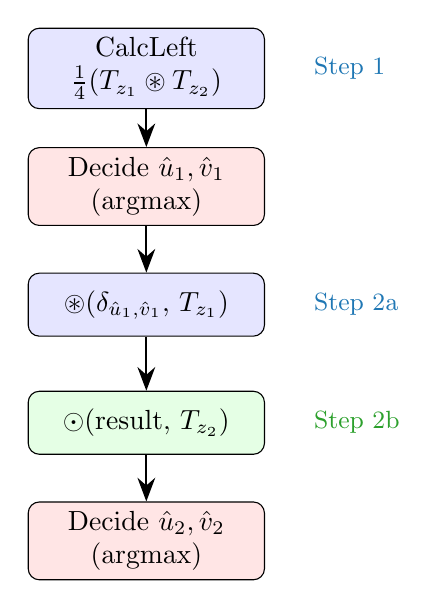
\begin{tikzpicture}[
    box/.style={draw, rounded corners, minimum width=3cm, minimum height=0.8cm, align=center},
    arrow/.style={-{Stealth[length=3mm]}, thick}
]
\node[box, fill=blue!10] (cl) at (0,0) {CalcLeft\\$\frac{1}{4}(T_{z_1} \conv T_{z_2})$};
\node[box, fill=red!10] (d1) at (0,-1.5) {Decide $\hat{u}_1, \hat{v}_1$\\(argmax)};
\node[box, fill=blue!10] (conv) at (0,-3) {$\conv(\delta_{\hat{u}_1,\hat{v}_1},\, T_{z_1})$};
\node[box, fill=green!10] (np) at (0,-4.5) {$\nprod(\text{result},\, T_{z_2})$};
\node[box, fill=red!10] (d2) at (0,-6) {Decide $\hat{u}_2, \hat{v}_2$\\(argmax)};

\draw[arrow] (cl) -- (d1);
\draw[arrow] (d1) -- (conv);
\draw[arrow] (conv) -- (np);
\draw[arrow] (np) -- (d2);

\node[right=0.5cm of cl, text=convblue] {\small Step 1};
\node[right=0.5cm of conv, text=convblue] {\small Step 2a};
\node[right=0.5cm of np, text=prodgreen] {\small Step 2b};
\end{tikzpicture}
\end{center}

%==============================================================
\section{Generalizing: The Tree for $N > 2$}
%==============================================================

For $N = 2^n$, the polar encoding is recursive: $n$ levels of XOR butterflies. The same two operations apply at every level of the tree.

\subsection{The Binary Tree}
\begin{center}
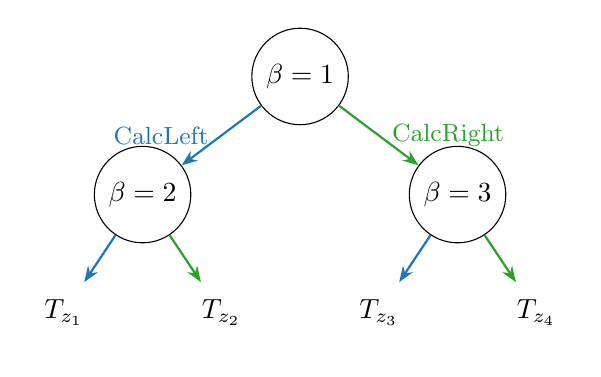
\begin{tikzpicture}[
    level distance=1.5cm, sibling distance=4cm,
    every node/.style={draw, circle, minimum size=0.6cm},
    edge from parent/.style={draw, thick, -{Stealth[length=2mm]}},
    level 2/.style={sibling distance=2cm}
]
\node {$\beta=1$}
    child { node {$\beta=2$}
        child { node[draw=none] {$T_{z_1}$} edge from parent[convblue] }
        child { node[draw=none] {$T_{z_2}$} edge from parent[prodgreen] }
        edge from parent[convblue] node[left, draw=none, text=convblue] {\small CalcLeft}
    }
    child { node {$\beta=3$}
        child { node[draw=none] {$T_{z_3}$} edge from parent[convblue] }
        child { node[draw=none] {$T_{z_4}$} edge from parent[prodgreen] }
        edge from parent[prodgreen] node[right, draw=none, text=prodgreen] {\small CalcRight}
    };
\end{tikzpicture}
\end{center}

At each internal node:
\begin{itemize}[nosep]
\item \textcolor{convblue}{\textbf{CalcLeft}} $\to$ left child: marginalizes unknown bits ($\conv$)
\item \textcolor{prodgreen}{\textbf{CalcRight}} $\to$ right child: incorporates decision ($\conv$ with $\delta$) + combines evidence ($\nprod$)
\end{itemize}

\subsection{Formal Definitions (Ren et al.\ 2025)}

Each edge in the tree carries a tensor (array of $2\times 2$ matrices). At vertex $\beta$ with parent edge $P$, left child $L$, and right child $R$:

\begin{tcolorbox}[colback=blue!5,colframe=convblue,title=CalcLeft (going down to left child)]
\[
L = P_{\text{first half}} \;\conv\; \big(P_{\text{second half}} \;\nprod\; R\big)
\]
First combine the second-half of parent with the right sibling ($\nprod$: independent evidence), then marginalize ($\conv$: XOR structure).
\end{tcolorbox}

\begin{tcolorbox}[colback=green!5,colframe=prodgreen,title=CalcRight (going down to right child)]
\[
R = P_{\text{second half}} \;\nprod\; \big(L \;\conv\; P_{\text{first half}}\big)
\]
First shift by the left child's decision ($\conv$ with decided values), then combine with parent's direct evidence ($\nprod$).
\end{tcolorbox}

\begin{tcolorbox}[colback=gray!5,title=CalcParent (going back up)]
\[
P = L \;\nprod\; R
\]
Combine both children's information ($\nprod$: two observations of the same variable).
\end{tcolorbox}

\textbf{Key insight:} At $N=2$, these reduce to exactly Steps 1 and 2 from our derivation. For larger $N$, the same operations apply recursively — the tree structure mirrors the recursive XOR encoding.

%==============================================================
\section{The Neural Replacement}
%==============================================================

\renewcommand{\arraystretch}{1.4}
\begin{center}
\begin{tabular}{lll}
\toprule
\textbf{Component} & \textbf{Analytical SC} & \textbf{Neural (NCG/NPD)} \\
\midrule
Representation & $2\times 2$ tensor & $d$-dimensional embedding \\
$T_{z_i}$ & $P(z_i \,|\, x, y)$ & $\text{MLP}(z_i) \to \mathbb{R}^d$ \\
CalcLeft ($\conv$ + $\nprod$) & Exact formula & $\text{MLP}(\text{concat}(e_{\text{parent}}, e_{\text{sibling}}))$ \\
CalcRight ($\nprod$ + $\conv$) & Exact formula & $\text{MLP}(\text{concat}(e_{\text{parent}}, e_{\text{left}}, u_{\text{sign}}))$ \\
CalcParent ($\nprod$) & Exact formula & Gated residual MLP \\
Decision & $\arg\max_{u,v}$ & $\text{MLP}(e) \to 4\text{-class logits}$ \\
\bottomrule
\end{tabular}
\end{center}

\bigskip

\textbf{Why go neural?}
\begin{itemize}[nosep]
\item The analytical decoder requires knowing $P(z_i \,|\, x, y)$ exactly.
\item For channels with \textbf{memory} (ISI, Ising, MA-AGN), the transition probabilities depend on previous inputs and hidden states — the exact tensor $T_{z_i}$ is unknown or intractable.
\item The neural $z$-encoder \textbf{learns} the channel embedding from samples, without requiring explicit channel knowledge.
\item The tree operations (CalcLeft, CalcRight, CalcParent) are replaced by MLPs that learn the correct transformations end-to-end.
\end{itemize}

%==============================================================
\section{Summary}
%==============================================================

\begin{tcolorbox}[colback=yellow!5,colframe=orange,title=The Complete Picture]

\textbf{Two primitives:}
\begin{enumerate}[nosep]
\item \textcolor{convblue}{$\conv$ (Circular Convolution)}: Marginalizes over unknown bits linked through XOR encoding. Answers: ``What do the observations tell us about the message bits?''
\item \textcolor{prodgreen}{$\nprod$ (Normalized Product)}: Combines independent observations about the same variable. Answers: ``Given two pieces of evidence, what is our combined belief?''
\end{enumerate}

\textbf{The tree:}
\begin{itemize}[nosep]
\item CalcLeft = $\conv$ + $\nprod$ (go down to left child)
\item CalcRight = $\nprod$ + $\conv$ (go down to right child, using decision)
\item CalcParent = $\nprod$ (go back up)
\item Applied recursively: $O(N \log N)$ total operations
\end{itemize}

\textbf{The neural extension:}
\begin{itemize}[nosep]
\item Replace $2\times 2$ tensors with $d$-dimensional embeddings
\item Replace exact $\conv$/$\nprod$ with learned MLPs
\item Preserves tree structure, works on unknown channels
\end{itemize}

\end{tcolorbox}

\end{document}
